\documentclass[conference]{IEEEtran}
\usepackage{cite}
\usepackage{amsmath,amssymb,amsfonts}
\usepackage{algorithmic}
\usepackage{graphicx}
\usepackage{hyperref}
\usepackage{textcomp}
\usepackage{xcolor}
\def\BibTeX{{\rm B\kern-.05em{\sc i\kern-.025em b}\kern-.08em
    T\kern-.1667em\lower.7ex\hbox{E}\kern-.125emX}}
\begin{document}

\title{Twitter Data Streaming, Sentiment Analysis, and Caching Recommendations\\}

\makeatletter
\newcommand{\linebreakand}{%
  \end{@IEEEauthorhalign}
  \hfill\mbox{}\par
  \mbox{}\hfill\begin{@IEEEauthorhalign}
}
\makeatother

\author{\IEEEauthorblockN{1\textsuperscript{st} Sidharth Bambah}
\IEEEauthorblockA{\textit{Electrical Engineering} \\
\textit{Columbia University}\\
New York, USA \\
sidharth.bambah@columbia.edu}
\and
\IEEEauthorblockN{2\textsuperscript{nd} Radhika Chinni}
\IEEEauthorblockA{\textit{Electrical Engineering} \\
\textit{Columbia University}\\
New York, USA \\
rpc2129@columbia.edu}
\and
\IEEEauthorblockN{3\textsuperscript{rd} Afam Nwokolo}
\IEEEauthorblockA{\textit{Electrical Engineering} \\
\textit{Columbia University}\\
New York, USA \\
kan2141@columbia.edu}
\linebreakand
\IEEEauthorblockN{4\textsuperscript{th} Christine Silveira}
\IEEEauthorblockA{\textit{Electrical Engineering} \\
\textit{Columbia University}\\
New York, USA \\
cs3876@columbia.edu}
\and
\IEEEauthorblockN{5\textsuperscript{th} Vedant Dave}
\IEEEauthorblockA{\textit{Electrical Engineering} \\
\textit{Columbia University}\\
New York, USA \\
vad2134@columbia.edu}
}
\maketitle

\begin{abstract}
Twitter has skyrocketed into a huge social media platform with tremendous amounts of users and data generated daily shifting Twitter's role into a content delivery network. This paper seeks to propose an effective content caching recommendation system by exploiting the hashtag structure of tweets and utilizing data stream processing to aggregate hashtag counts and generate popularity distributions. Additionally, an extension is presented to use the streaming software in conjunction with machine learning for accurate sentiment analysis.
\end{abstract}

\begin{IEEEkeywords}
content distribution networks, Twitter, streaming, Spark, BigQuery, Dataproc
\end{IEEEkeywords}

\section{Introduction}
In the past few years, Twitter has become a dominant social media platform with a skyrocketing amount of users. At its core, Twitter is a micro-blogging platform that allows users to write "tweets" within roughly 280 characters. \par

This growth has led to Twitter becoming a content delivery network (CDN) in its own right. Once tweets are generated, users are able to search for content of interest. This leads to interesting new problems for Twitter. Particularly, the entire network must have a means to effectively cache the most popular tweets for quick retrieval. Additionally, the popularity of tweets shifts dynamically with human sentiment and sociopolitical events. \par

Further, tweets are generated dynamically on a temporal scale based on user activity. Thus, it is important to be able to process the data quickly as it comes in. The streaming nature of the data makes it difficult to store entire tweets and parse through them. Rather, this paper proposes an approach to process important sections of tweets as they come in without storing the entire tweet. In essence, tweets can be analyzed with straightforward data analytic tools that collect and batch process data elements that come in through time. \par

This paper also outlines a method to develop machine learning models that tweets can act on for purposes of sentiment analysis and opinion mining. As will be seen, this field has an immense potential that can start to be tapped with highly accurate models, which can now be made due to the colossal amount of data generated by Twitter's users. \par

\section{Motivation}
Twitter receives a massive amount of tweets daily. Each tweet consists of one or more hashtags, which serve as keywords for the content contained in the tweet. With this layout, users can easily search for content of interest based solely on a hashtag. However, each user search based on hashtag can be quite expensive without an effective way to cache the most likely to be accessed tweets. Therefore, a method of tweet popularity classification will be essential for Twitter's effective operation as a content delivery network. \par

The anatomy of the tweet as seen in Figure \ref{fig:tweet_anatomy} can be exploited for use with data streaming processing tools. In essence, the content following a hashtag can be recorded for each incoming tweet and counted. This allows for dynamic calculation of hashtag frequency, which strongly correlates to popularity. After storing the counts of hashtags over a specified streaming window, visualizations can be generated to provide useful caching recommendations. \par

\begin{figure}
    \centering
    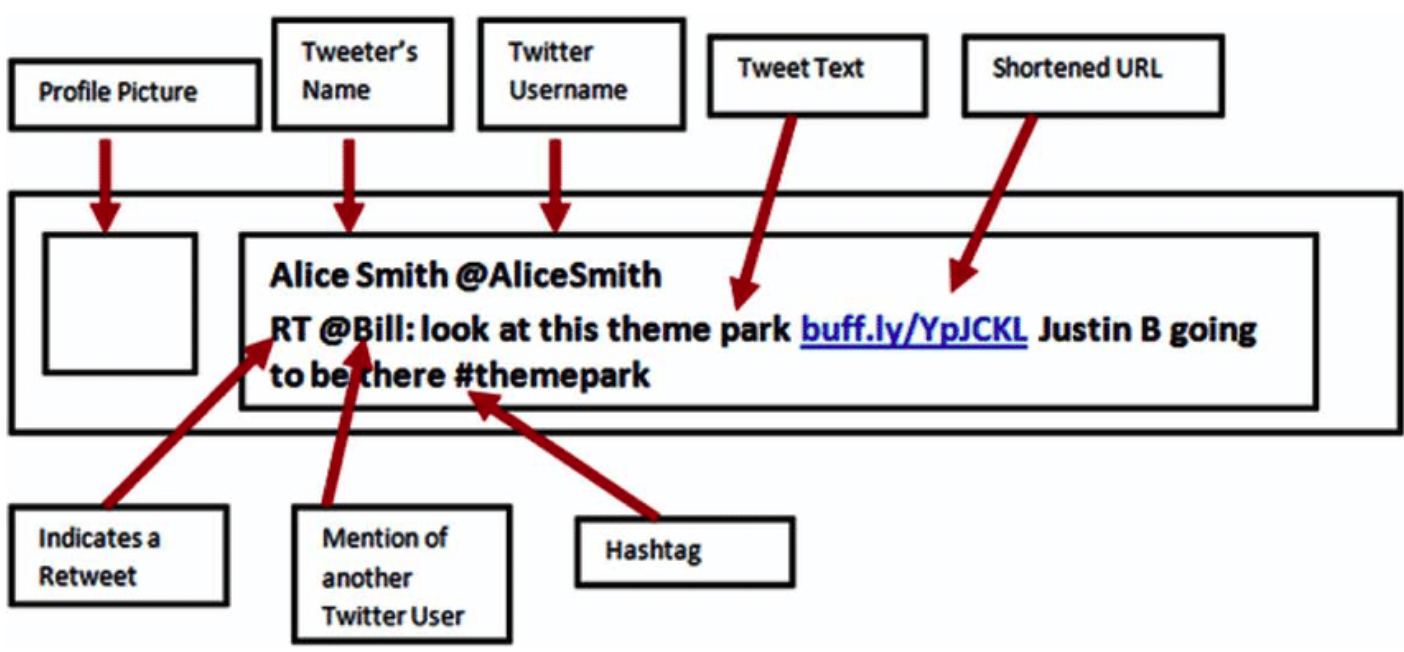
\includegraphics[scale=0.5]{img/tweet_anatomy.PNG}
    \caption{Anatomy of a Tweet. Hashtags can be used for data stream processing in batches over specified stream length. Adapted from \cite{tweet_anatomy_figure}.}
    \label{fig:tweet_anatomy}
\end{figure}

If Twitter implements a caching scheme based on hashtag count, only the most popular tweets will be cached. This will allow for fast tweet look-ups and efficient search queries from users. It is important to note that hashtag counts must be periodically refreshed as popularity is constantly shifting based on user input. \par

\section{Implementation}

\subsection{Overview}
Tweets come in unpredictably and cannot be effectively analyzed in post-processing. This variable nature makes Twitter posts well-suited to stream processing techniques. \par

A popular method to process data streams is with Apache Spark, which allows for low latency analytics of streaming traffic data. Furthermore, Spark allows for real-time and periodic-batch analysis with minimal overhead \cite{7364101}. Additionally, Spark maintains linear scalability and fault tolerance while providing a rich Python API built on the core abstraction of a distributed data frame \cite{Shanahan:2015:LSD:2783258.2789993}. This is quite essential as each tweet must be processed quite quickly as it arrives and is only seen once. Essentially, words following a hashtag can be aggregated and linearly projected into counts. \par

\subsection{Program}

The overarching software architecture used to design the Twitter data streaming and hashtag counting program can be seen in Figure \ref{fig:software_architecture}.

\begin{figure}
    \centering
    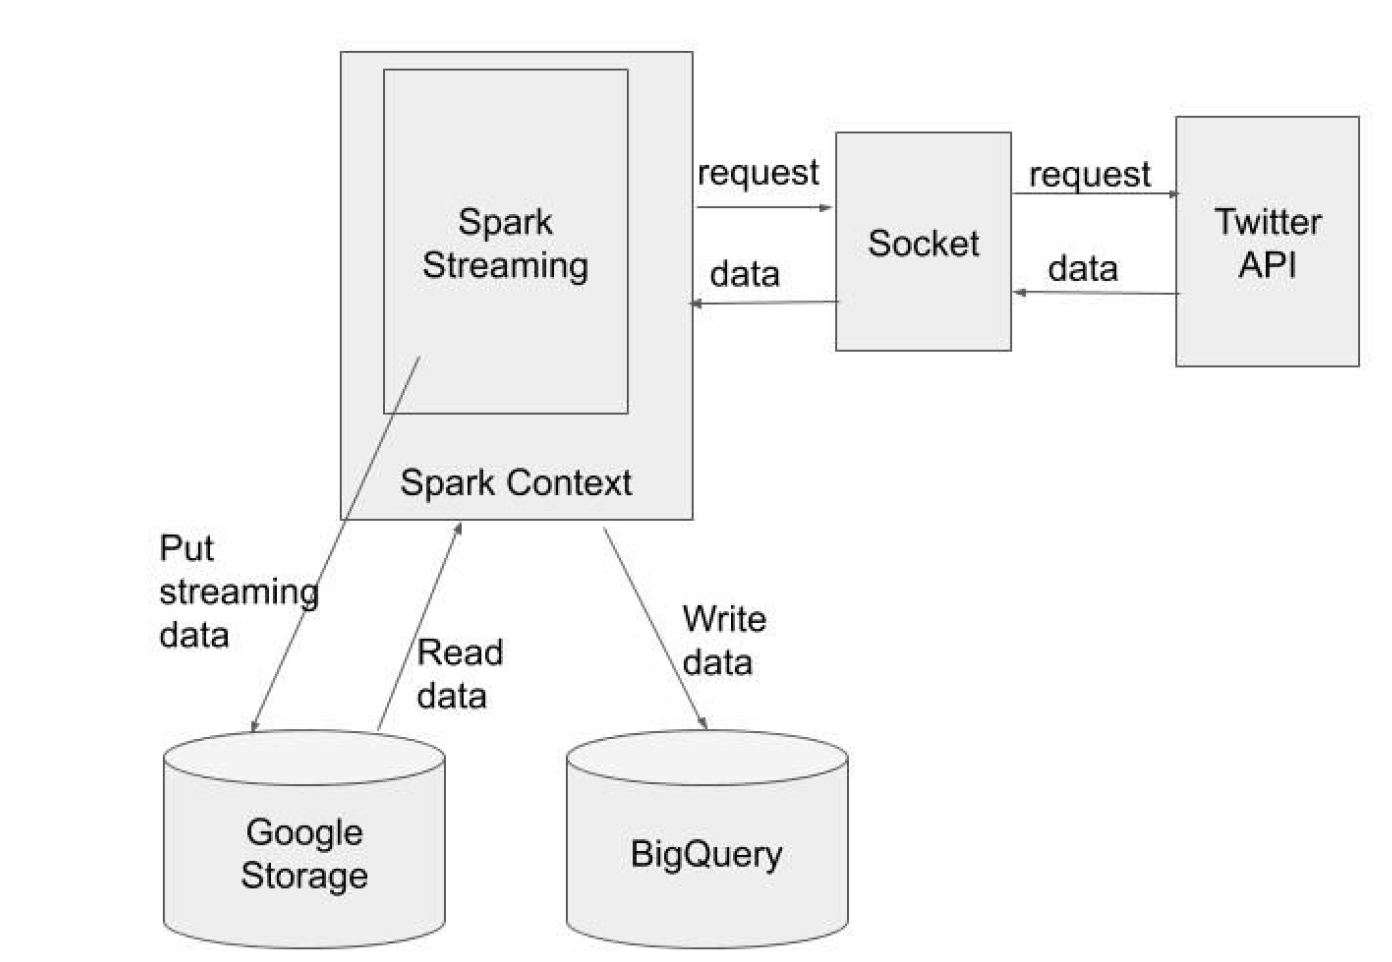
\includegraphics[scale=0.5]{img/software_architecture.PNG}
    \caption{The software architecture structure for the Twitter hashtag counting program. Apache Spark is used for all data stream processing. Google Storage is employed for intermediate data storage. BigQuery SQL database is used for storing the final hashtag table.}
    \label{fig:software_architecture}
\end{figure}

In the following implementation, Twitter issues a developer key that allows for API level access. Clearly, Twitter is performing a role as a content delivery network by allowing access to the streaming data created by user tweet generation. For this implementation, Twitter only issued a standard API key rather than a commercial key. One important note is that the standard key requires that all streaming clients define a set of tags, which are tracked when the tweets are received. Thus, only a subset of the entire tweets were used for this paper. The tags were chosen as follows for relevance: ['\#', 'content', 'delivery']. After taking note of these limitations, python's HTTP socket handler and the "tweepy" Twitter API client allowed for easy access to the live data streams generated by Twitter's users. \par

After the HTTP socket program is running, as can be seen in Figure \ref{fig:http_client}, another Python program runs and connects to the socket over a TCP port. All of the data is subsequently streamed into an Apache Discretized Stream (Dstream) object, which allows for batch processing of the data as well as transformations and mappings given a certain window size and streaming interval. \par

\begin{figure}
    \centering
    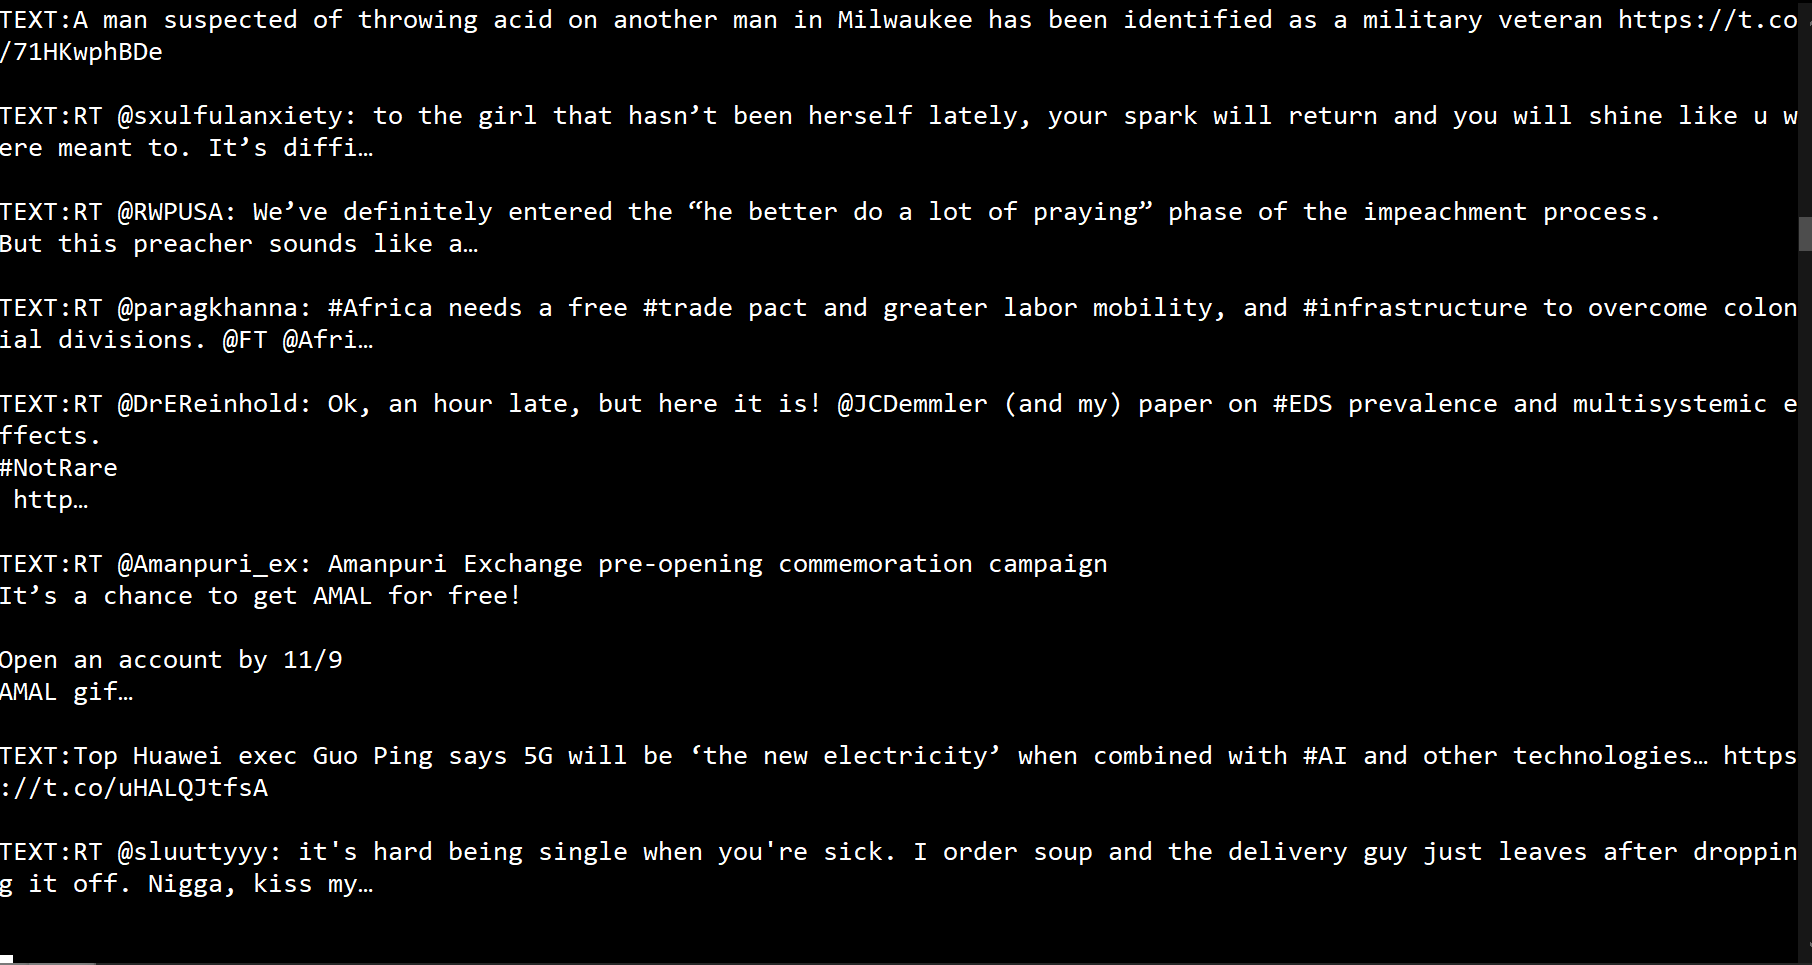
\includegraphics[scale=0.35]{img/http_client.PNG}
    \caption{Running socket program that reads streaming tweets using the Python 'tweepy' library. Connected directly to Twitter's API and tracking select words.}
    \label{fig:http_client}
\end{figure}

Once the tweet content is streaming, it is essential to clean and parse the data for efficient analysis. The first step is to set all of the characters to lower case allowing for easy aggregation. Upon cleaning, all words following a '\#' character are saved into the system's cache. Not that, for the purposes of this implementation, all hashtags with non-alphanumeric characters are dropped. \par

After each window length, the hashtags are aggregated and projected into a count. This means that all hashtags are initially given a count of 1. Then, they are grouped word and the counts of all grouped elements are summed. This process can continue over any period length, but it is quite CPU intensive to process incoming data continuously. Hence, this simulation is run for a period of 20 minutes. Sample output of the hashtag aggregation program can be seen in Figure \ref{fig:hashtag_aggregation} \par

\begin{figure}
    \centering
    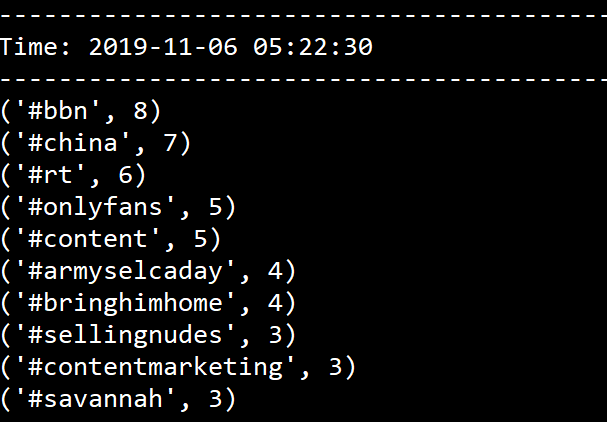
\includegraphics[scale=1.0]{img/hashtag_aggregation.PNG}
    \caption{Output of second script which is connected to the socket opened by the first. The spark Dstream object are being batch processed and the hashtag counts are projected into a sum.}
    \label{fig:hashtag_aggregation}
\end{figure}

As the program runs, intermediate data from each aggregated Dstream object is written into a Google Storage bucket. Due to the low latency of reading and writing from the bucket, this is akin to storing the data in cache. \par

As soon as the simulation ends, the data is written to a relational SQL database and the temporary files are purged from the Google Storage bucket. Once in the database, queries can be run to order the hashtag values by count and find out which are the most popular. Additionally, visualizations can be created to show the percentage of certain hashtags as well as raw values. These results can then be used to programmatically rank hashtags based on frequency and provide popularity distributions that directly correspond to caching recommendations. \par

\subsection {System}

The entire system architecture can be seen in Figure \ref{fig:system_architecture}. For simplicity, all of the cloud computing resources are provided from Google Cloud with a student license.

\begin{figure}
    \centering
    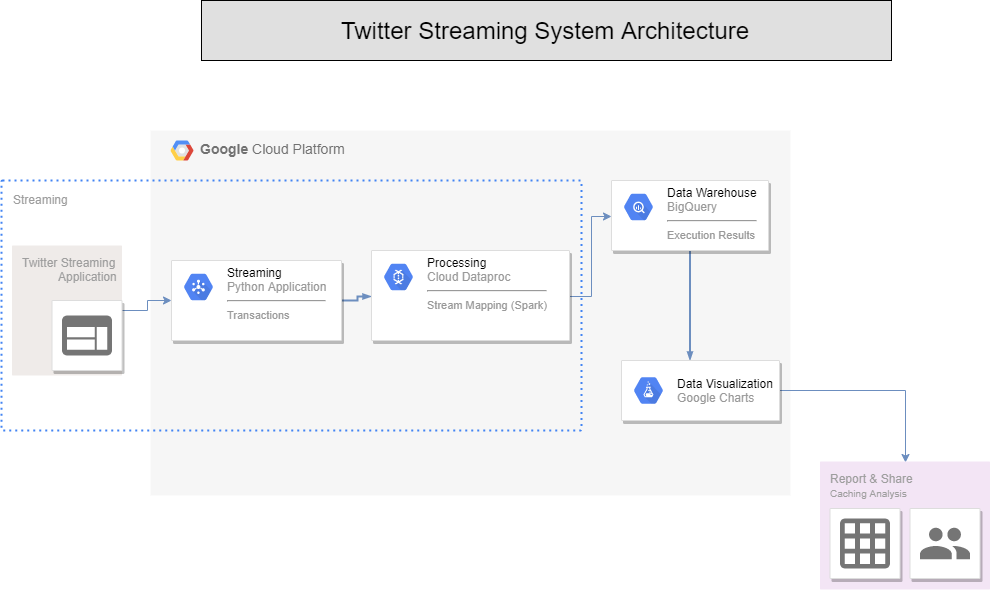
\includegraphics[scale=0.25]{img/system_architecture.png}
    \caption{All of the components for the Twitter streaming application. Computation and analysis are done in Dataproc clusters and BigQuery while visualizations are rendered with Google Charts.}
    \label{fig:system_architecture}
\end{figure}

In this implementation, both scripts were run on a Google Cloud Dataproc cluster with 2 master nodes and 2 worker nodes. The cluster allows for scalable computing resources and fast computation over large datasets. Additionally, these clusters are optimized for the Apache Spark library and also have instances of Jupyter notebook, which were critical for testing, debugging, and quick visualizations for simple analysis. \par

In order for easy integration with the Google Dataproc cluster, this system heavily relies on Google's BigQuery database platform. BigQuery is a SQL database that is optimal for large datasets and allows for easy queries. A subset of the data recorded into BigQuery for the first run of the software is given in Figure \ref{fig:bigquery_table}. \par

\begin{figure}
    \centering
    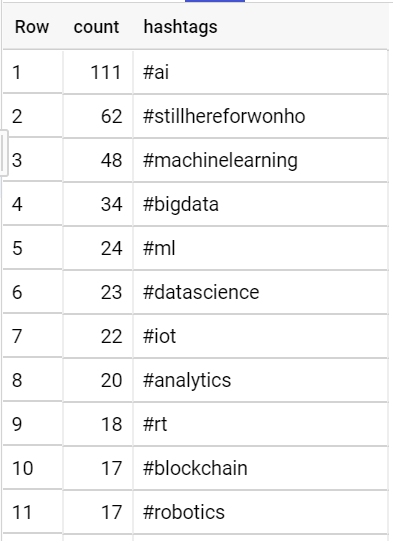
\includegraphics[scale=0.7]{img/bigquery_table.PNG}
    \caption{Subset of the hashtag table stored in BigQuery. As expected, the most common results are from those elements tracked due to the Twitter API limitation.}
    \label{fig:bigquery_table}
\end{figure}

Lastly, the pandas library with its dataframe objects is essential for visualization development. A typical structured dataset comes in a tabular format and pandas allows this table to be stored as a collection of independent columns in a dataframe object \cite{pandas_summary}. Operations can be performed on dataframes to mutate the data and pull out meaningful results. One significant mutation is a sorting algorithm implemented in dataframes. As can be seen from Figure \ref{fig:bigquery_table}, the hashtags table contains a counts column. To generate useful results, it is important to sort the results by the count in a descending order. This can be done quite easily with Pandas dataframe objects. Additionally, slices of data, such as the top 10 hashtags, can be pulled out an analyzed with low overhead. \par

By querying BigQuery and extracting the data into a dataframe, the hashtags and frequencies can be easily filtered and manipulated. Additionally, the Plotly graphing library for Python can be used in a Google Colab notebook to render the data into many different visual elements including, but not limited to, scatter-plots, bar-plots, histograms, pie charts, and donut charts. \par

\section{Results}
The software written for the above implementation was run two times to generate two distinct datasets. The runs were performed on two different days 4:30PM Eastern Standard Time on each day. This is done to capture shifting human emotions over time.  \par

Upon collecting the data from twenty minutes of streaming for each of these cases, visualizations were rendered using Google Charts to accurately interpret the data and determine which hashtags were the most popular at the time. This popularity distribution over hashtags can be used to make reliable caching predictions for Twitter. \par

As expected, the received hashtags are strongly correlated with the tracked tags as mentioned in the system design. This is due to the lack of "firehose" access from Twitter limiting the amount of tweets that can be accessed in a streaming session. \par

\subsection{First Run}
In the first twenty minute run of the software on November 7, 2019 starting at 4:30PM Eastern Standard Time, the results given in Figures \ref{fig:bar_run1} and \ref{fig:donut_run1} were generated. The software resulted in 842 distinct hashtags and only the 10 with the highest counts appear in this analysis. \par

The bar graph in Figure \ref{fig:bar_run1} gives a clear view of the counts of the ten most popular hashtags users generate in the twenty minutes of streaming. Based on these results, \#content and \#gift are the two most popular hashtags. \par

Similarly, the donut chart, gives a visual representation of how much of the whole each hashtag makes up. It seems that there are no outliers which disproportionately affect the graph. This means that all of these popular hashtags can and should be cached in a similar manner without any weighting aside from their frequencies. \par

The fact that \#content is one of the most popular makes sense since the tweets with the words 'content' in them are tracked due to the API restrictions. However, beyond this, it is also reasonable that \#gift is the second most frequent tag due to the holiday season in happening during the time the data was recorded. Thus, it follows that tweets with holiday motifs should be cached at this time. \par

\begin{figure}
    \hspace*{-1cm}
    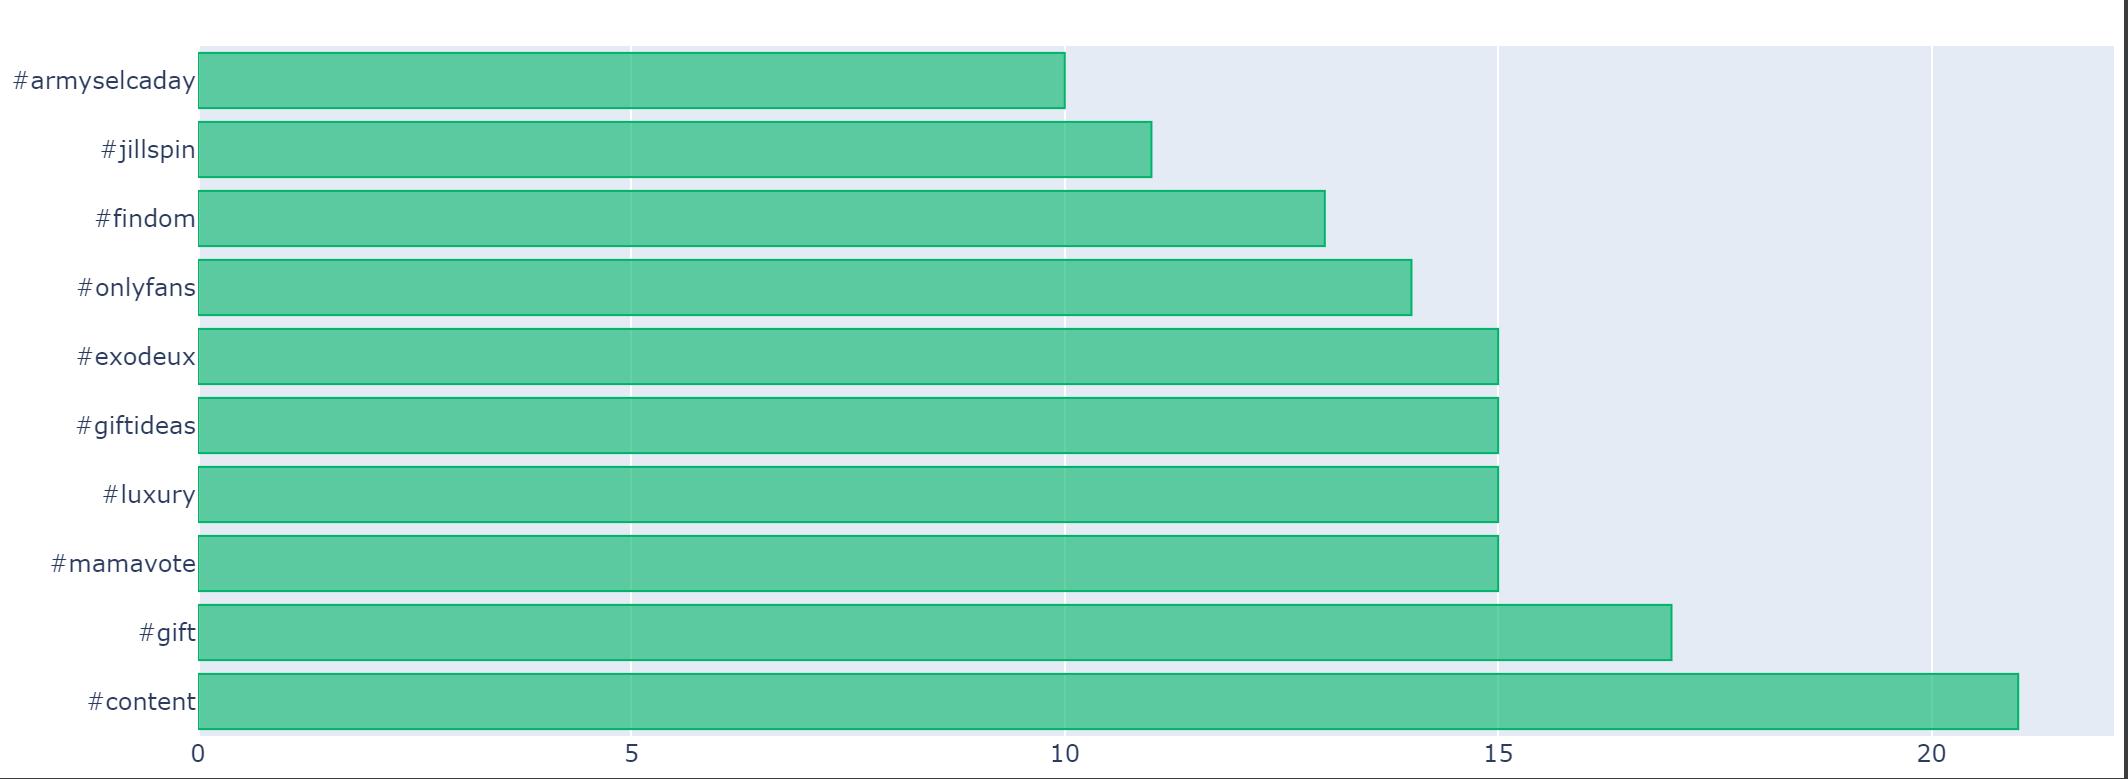
\includegraphics[scale=0.35]{img/bar_run1.PNG}
    \caption{Bar graph of the raw values for top ten hashtags collected during the first software run at 4:30PM on November 7, 2019.}
    \label{fig:bar_run1}
\end{figure}

\begin{figure}
    \hspace*{-1cm}
    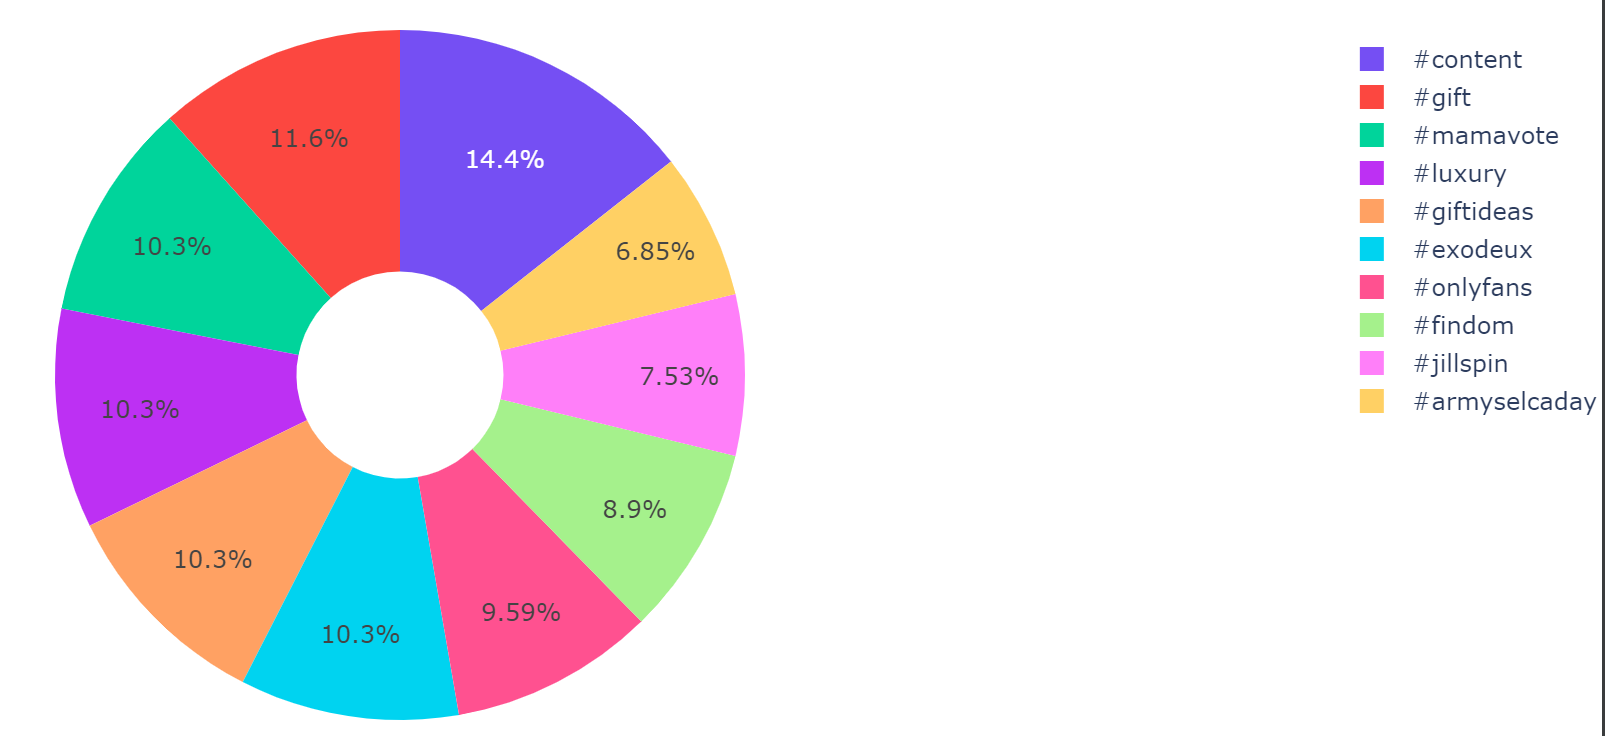
\includegraphics[scale=0.45]{img/donut_run1.PNG}
    \caption{Donut graph of frequency distribution for the hashtags collected during the first software run at 4:30PM on November 7, 2019.}
    \label{fig:donut_run1}
\end{figure}

\subsection{Second Run}
In the second twenty minute run of the software on December 7, 2019 starting at 11:00AM Eastern Standard Time, the results given in Figures \ref{fig:bar_run2} and \ref{fig:donut_run2} were generated.

Based on the bar graph in Figure \ref{fig:bar_run2}, it seems that in this second run, \#lay and \#kiisjingleball are the most popular hashtags. \par

Similarly, the donut chart representation shows that \#lay is an outlier that disproportionately affects the rest of the graph. Thus, if this were normalized to a standard, cachine recommendations could be more effectively made. \par

As can be seen, the time of day as well as the time of year makes a large difference on the results of the streaming data collection. This is due to the ever-shifting human sentiment. Thus, this phenomenon must be accounted for in any caching algorithm. This can be done by periodic updating. Perhaps, collections can be made on a weekly basis. \par

\begin{figure}
    \hspace*{0cm}
    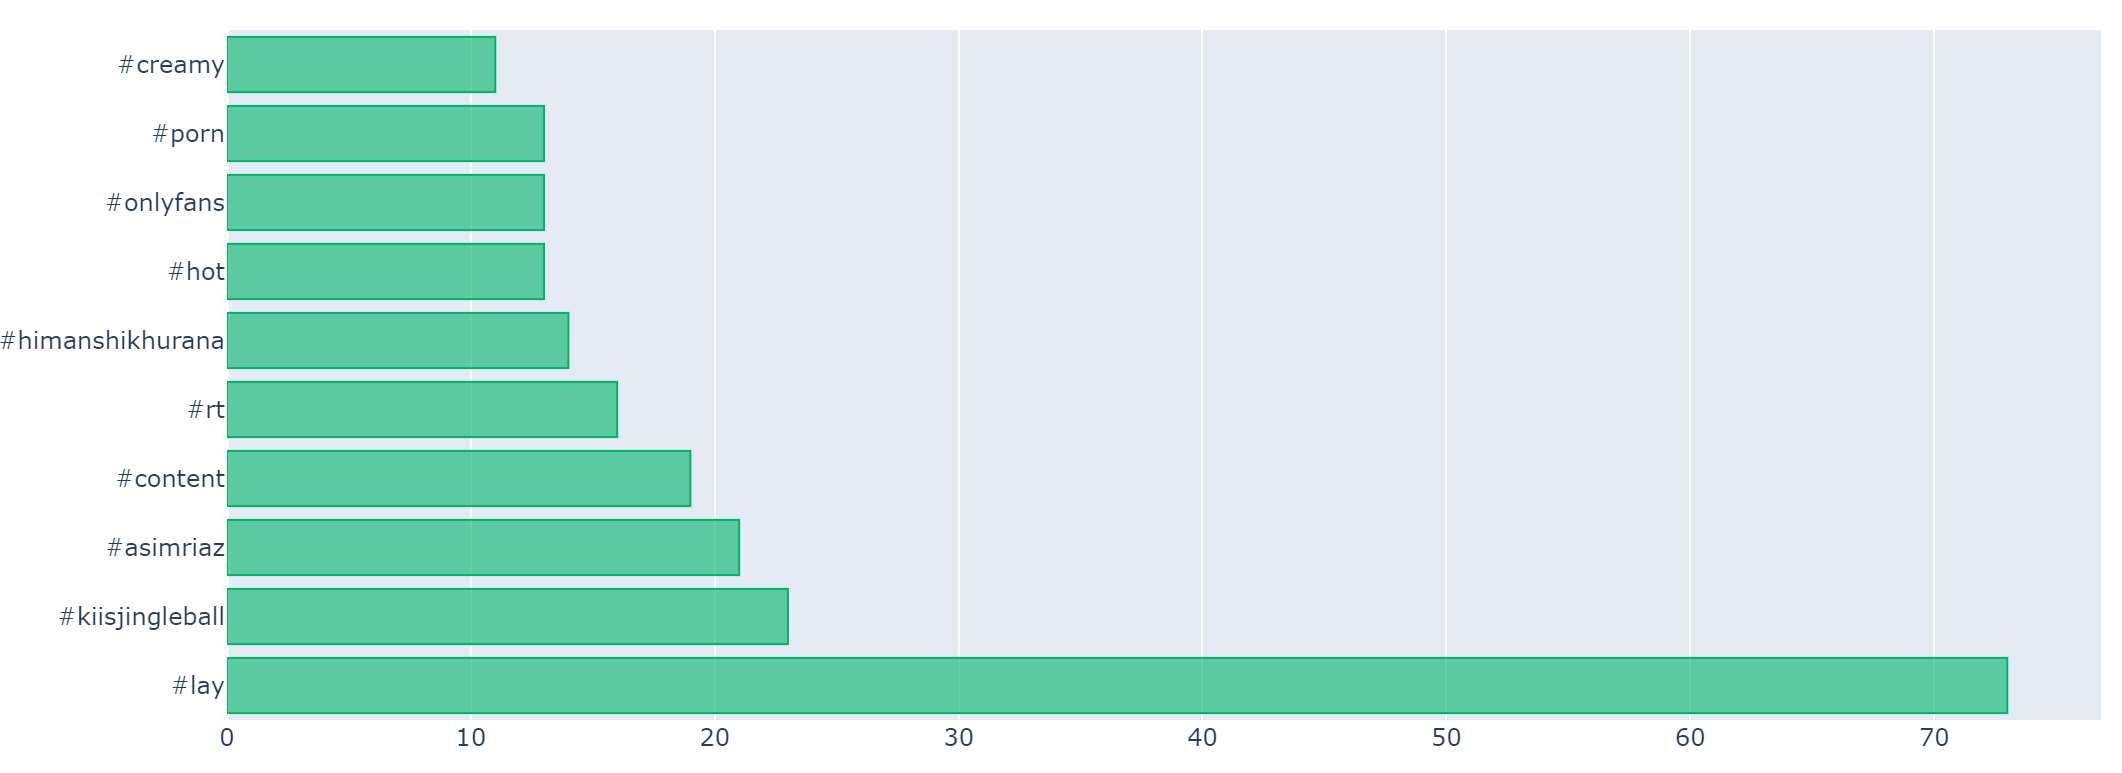
\includegraphics[scale=0.35]{img/bar_run2.PNG}
    \caption{Bar graph of the raw values for top ten hashtags collected during the second software run at 11:00am on December 7, 2019.}
    \label{fig:bar_run2}
\end{figure}

\begin{figure}
    \hspace*{0cm}
    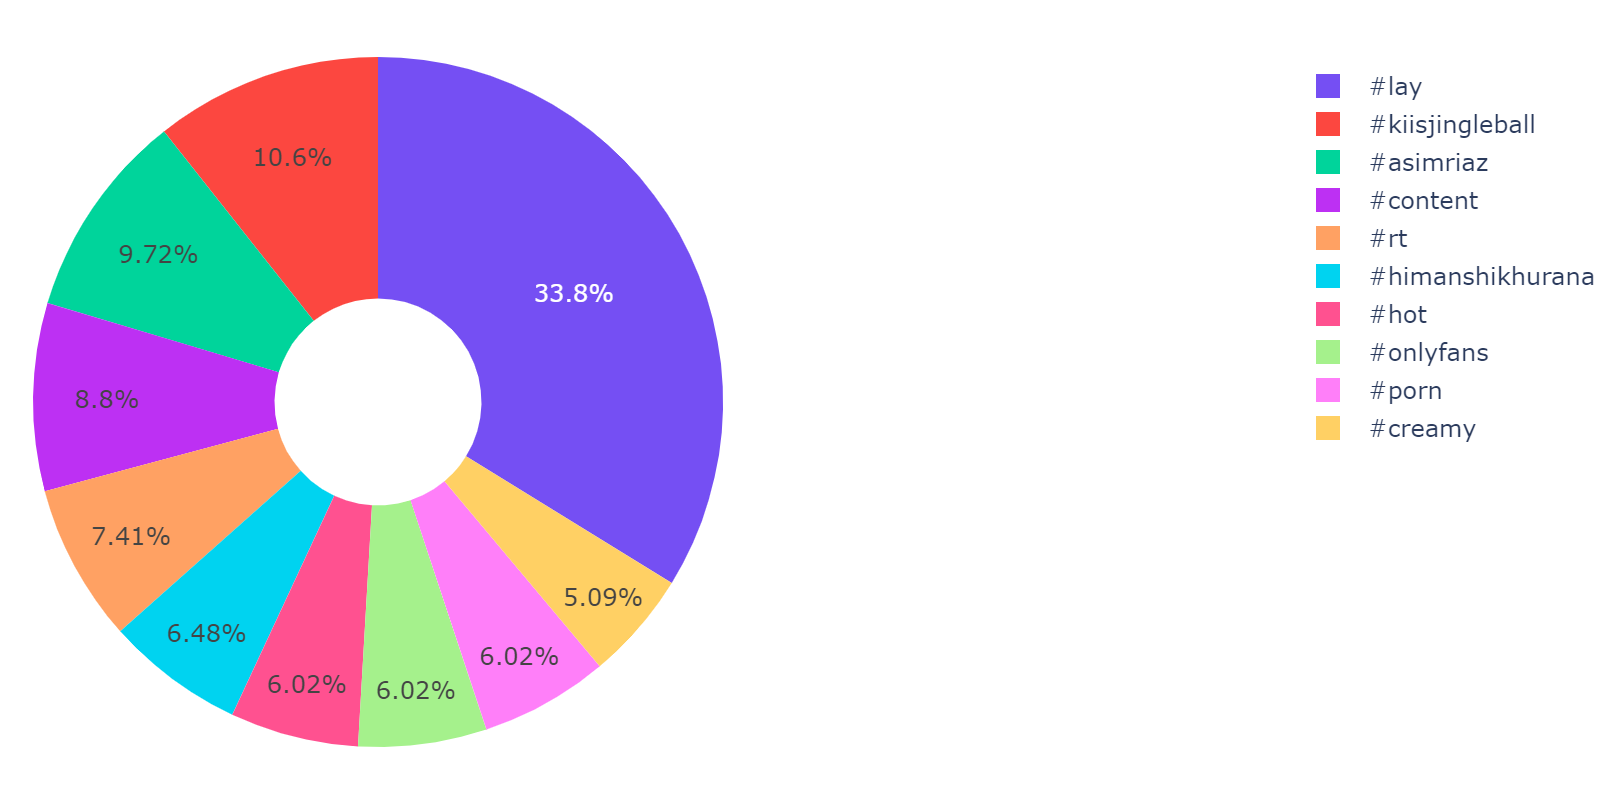
\includegraphics[scale=0.45]{img/donut_run2.PNG}
    \caption{Donut graph of frequency distribution for the hashtags collected during the second software run at 11:00AM on December 7, 2019.}
    \label{fig:donut_run2}
\end{figure}

\section{Sentiment Analysis}
The field of machine learning and artificial intelligence offers a means for sentiment analysis, which can have a tremendous impact. \par

By extracting the hashtag data stored in BigQuery, the words can be cleaned and parsed using Natural Language Processing (NLP) tools. Then, machine learning models can be developed to aid in understanding sentiments contained in each hash tag. As with any model, certain features must be identified and trained on a set of data. For the purpose of sentiment analysis, features can be split into three major categories: lexicon features, part-of-speech features, and micro-blogging features. \par

Lexicon features are based on the dictionary definitions of words and their tagging, which can be positive, negative, or neutral. Part-of-speech features include verbs, adverbs, adjectives, nouns, and other parts of speech. Lastly, micro-blogging features include emoticons, abbreviations, and intensifiers, such as all-caps and character repetitions \cite{sentiment_kouloumpis}.

Once these features are compiled, it is important to perform some exploratory analysis on the dataset. In this case, the dataset would be a compilation of historical Twitter tweets ranging back at least a few years. Here, it is quite important to note that the huge amount of data Twitter has available in the form of user generated tweets yields the opportunity to create highly accurate predictive models. \par

One particularly useful exploratory tool is a correlation matrix. This will reveal strong associations between features and provide insights as to which type of machine learning model would be best suited for the data. Additionally, scatter plots can be generated to find linear relationships between the data as well as possible clusters that may have naturally formed. \par

Recently, the most common machine learning models have been in the form of neural nets; however, there are numerous other, oftentimes simpler, models, such as random forests and binary classifiers, which may be better fits for the data. Another fundamental approach, which is likely to yield a high accuracy, is the Naive Bayes classifier. This method is used in a closely related work and is effective due to it's supervised learning framework. Using the adaptation of the Naive Bayes formula given in Equation \ref{eqn: naive_bayes}, tweets can be classified into the right category based on a set of pre-classified tweets. Here, class $c$ is assigned to each individual tweet $d$ and $f$ represents a feature while $n_i(d)$ represents the count of feature $f_i$ in tweet $d$ \cite{6897213} \par

\begin{equation}
P_{NB}(c\vert d):={\frac{(P_{(c)})\Sigma_{i=1}^{m}P(f\vert c)^{n}i^{(d)}} {P(d)}}
\label{eqn: naive_bayes}
\end{equation}

Regardless of the model chosen, the historical data must be split into a test and training set. Then, the model will be trained with the training portion of the data and evaluated on the test set. Once a suitable accuracy is achieved, the model can be deployed. \par

After a model with the required accuracy is deployed, a stream of incoming Tweets can be dynamically run against the model based on the filtered hashtags. Next, each hashtag can be assigned a so-called "toxicity score", which determines the level of rudeness or offensiveness present in the hashtag. Additionally, hashtags can be further grouped based on opinions and can be used to roughly determine amounts of users who believe or agree with certain things. \par

This approach to sentiment analysis also opens room for non-technical studies into the broader implications of such opinion mining. Particularly, there are questions of privacy, the data's vulnerability to manipulation, and whether or not mined sentiments can have any measurable economic impact \cite{pang_lee_2008}. \par

\section{Extensions}
This method for Twitter caching recommendations has significant scope for extension. \par

More broadly, the popularity distribution of hashtags can be used to optimize caching in traditional content distribution networks as well. Online Social Networks (OSNs), such as Twitter, represent a large fraction of global Internet traffic. However, this has led to a rise of User Generated Content (UGC), which has  a long-tailed popularity distribution with a large number of low popularity items and few popular ones. The hashtag information, along with other aspects of the tweet, such as the user himself and his followers, can be used to classify content into different interest categories based on social relationships, common interests, and locality of content exchange. This classification can constitute new metadata information, which has the potential to allow for the implementation of distributed caching systems with only relevant content at each node \cite{6932933}. Currently, OSNs tend to outsource their content to CDN services, such as Akimai, or end up becoming delivery networks themselves; this approach allows for both the OSN and CDN service to work in conjunction to develop caching mechanisms with high hit ratios. \par

Aside from web CDN caching optimization use cases, if the hashtag popularity distribution were to be released to the public, there would surely be many interesting applications of the data in the fields of affiliated marketing, business analytics, advertisement, and even politics. Clearly, there is a huge scope for the streaming data generated by OSNs, with Twitter in particular. However, all of these applications are largely dependent on the opening of data streams for public consumption to propel innovation. \par

\section{Conclusion}
Since its inception, Twitter has revitalized the social media sphere. The micro-blogging platform's novel hashtag scheme and concise tweet size limitations has led to a proliferation of user generated content. This has thrust Twitter into the role of a content delivery network with its robust streaming API, search algorithms, and hashtag sorting mechanisms. \par

As such, it is imperative for Twitter to successfully cache the most frequently accessed tweets. This paper aims to provide a multi-faceted approach to effectively count the frequency of hashtags from the streaming data using batch processing and linear projection methods. With this information, visualizations can be prepared to analyze the collected data and determine popularity distributions for the hashtags. These distributions directly correlate to the most frequently accessed tweets and provide crucial information that can be used to formulate an effective caching algorithm for Twitter. As mentioned, the caching algorithm will need to be periodically re-factored to take into account shifting human sentiment and variable popularity distributions for hashtags. \par

Along with efficient and dynamic caching based on hashtag count, the software written for this paper can have a crucial impact in terms of sentiment analysis for live tweets. If Twitter is able to release historical tweet information, that dataset coupled with existing word toxicity classifications, can be used to generate accurate, high-performance machine learning models to directly classify tweets and determine sentiments. As with the caching system, the models will need to be continuously updated with the latest information to maintain a high level of accuracy. \par

\section*{Acknowledgment}
The authors gratefully acknowledge the contributions of Professor Anwar Walid of the Electrical Engineering department at Columbia University and ELENE6776 TA Shanglin Guo for their insightful input and analysis leading to the creation of this work.


%\begin{thebibliography}{00}
%%%% Adding the bibliography from external file
\nocite{*}
\bibliographystyle{IEEEtran} % We choose the "IEEEtran" reference style
\bibliography{references} % Entries are in the "references.bib" file
%\end{thebibliography}

 \appendices

\section{Links}
The source code created in the development of this project can be found on GitHub at \url{https://github.com/SidBambah/Twitter-Streaming}. \par

\vspace{12pt}

\end{document}
